%
\documentclass[%
 reprint,
 amsmath,amssymb,
 aps,
]{revtex4-1}

\usepackage{graphicx}% Include figure files
\usepackage{dcolumn}% Align table columns on decimal point
\usepackage{bm}% bold math


\begin{document}


\title{Comparativa Datawarehouse vs DataLakes}
\author{Robles Flores, Anthony Richard	               (2016056192)}
\author{Estrella Palacios, Katherine Lizbeth			(2015050948)}
\author{Sosa Bedoya, Sharon Fiorela					(2016054460)}
\author{Torres Beltran , Johanna Andrea				(2020067849)}

		
\affiliation{%
 Universidad Privada de Tacna \textbackslash Facultad de Ingenieria \textbackslash Escuela Profesional de Ingenieria de Sistemas
}%

\begin{abstract}
\begin{center}
\textbf{Resumen}
\end{center}
Realizar la comparación entre Data Lake y Data Warehouse es algo muy común entre aquellas empresas que se disponen a implantar soluciones de big data. Una de las diferencias que marcan la comparación entre Data Lake vs Data Warehouse es que, este último, por lo general, sigue una metodología como las definidas por Inmon y Kimball, a diferencia de Data Lake.
\\

\begin{center}
\textbf{Abstract}
\end{center}
Making the comparison between Data Lake and Data Warehouse is very common among those companies that are preparing to implement big data solutions. One of the differences that make the comparison between Data Lake vs Data Warehouse is that the latter, generally, follows a methodology such as those defined by Inmon and Kimball, unlike Data Lake.
\\
\end{abstract}



\maketitle

%\tableofcontents

\section {Introducción}\label{sec:1}

Por mucho tiempo, los datawarehouses funcionaron como depósitos fundamentales de datos integrados que facilitaron las decisiones informadas. En el pasado reciente, el campo de la gestión de datos ha sido testigo de un cambio catastrófico con la llegada de Big Data que ha creado la necesidad de procesar un gran volumen y variedad de datos junto con el deseo de un acceso más rápido a los datos.
Datalakes se emplea ampliamente para cumplir con estos requisitos y se promociona como una ventana única para cumplir con todos los requisitos de datos de una organización. Esta suposición ha cuestionado el papel del Datawarehouse tradicional. Este documento describe las características esenciales de los datawarehouses y datalakes. También compara y contrasta los dos sistemas y concluye que los dos no son tecnologías competidoras sino complementarias. Juntos pueden atender de manera efectiva y eficiente las necesidades de gestión de datos de una organización.

%-----------------------------------------------------------------
\section{Objetivos}\label{sec:2}
\subsection{General:}
Dar una visión clara de BI, desde las perspectivas de los autores que sentaron las bases que son Ralph Kimball y Bill Inmon, para la mejora de las estrategias del negocio al que se desee implementar las herramientas de BI.
\subsection{Específicos:}
 Describir las metodologías propuestas por los principales autores de BI desde las perspectivas de sus creadores Ralph Kimball y Bill Inmon.


%-----------------------------------------------------------------
\section {Marco Teórico}

\subsection{DATAWAREHOUSE}	
Un Data Warehouse es una base de datos corporativa en la que se integra información depurada de las diversas fuentes que hay en la organización. Dicha
información debe ser homogénea y fiable, se almacena de forma que permita su análisis desde muy diversas perspectivas, y que a su vez dé unos tiempos de
respuesta óptimos. Para ello la información se encuentra altamente desnormalizada y modelada de una forma bastante diferente a los sistemas transaccionales,
principalmente se utilizan los modelos en estrella (star schema) y en copo de nieve (snowflake schema).\cite{robles3}

\subsubsection{Características DataWarehouse}	

Un Data Warehouse es mucho más que lo que hemos comentado hasta el momento. Según Bill Inmon se caracteriza por ser:
\begin{itemize}
	\item \textbf{Orientado a temas:}  los datos están organizados por temas para facilitar el entendimiento por parte de los usuarios, de forma que todos los datos relativos a un mismo elemento de la vida real queden unidos entre sí. Por ejemplo, todos los datos de un cliente pueden estar consolidados en una misma tabla, todos los datos de los productos en otra, y así sucesivamente.
	\item \textbf{Integrado:}  los datos se deben integrar en una estructura consistente, debiendo eliminarse las inconsistencias existentes entre los diversos sistemas operacionales. La información se estructura en diversos niveles de detalle para adecuarse a las necesidades de consulta de los usuarios. \\Algunas de las inconsistencias más comunes que nos solemos encontrar son: en nomenclatura, en unidades de medida, en formatos de fechas, múltiples
	tablas con información similar.
	\item \textbf{Histórico (variante en el tiempo):}   los datos, que pueden ir variando a lo largo del tiempo, deben quedar reflejados de forma que al ser consultados reflejen estos cambios y no se altere la realidad que había en el momento en que se almacenaron, evitando así la problemática que ocurre en los sistemas operacionales, que reflejan solamente el estado de la actividad de negocio presente. Un Data Warehouse debe almacenar los diferentes valores que
toma una variable a lo largo del tiempo. 
	\item \textbf{No volátil:}   la información de un Data Warehouse, una vez introducida, debe ser de sólo lectura, nunca se modifica ni se elimina, y ha de ser permanente y  mantenerse para futuras consultas. \\

Adicionalmente estos almacenes contienen metadatos (datos sobre los datos), que aportan un valor adicional, permitiendo tener información sobre su procedencia (sobre todo cuando tenemos múltiples fuentes), la periodicidad con la que han sido introducidos, la fiabilidad que nos ofrecen, etc. Todo ello nos aporta una ayuda adicional, tanto al usuario final como a los técnicos responsables de su mantenimiento, ayudando a estos últimos en aspectos como su auditoría y administración. \\

Kimball determinó que para él un Data Warehouse no era más que un conjunto de los Data Marts de una organización. Un Data Mart es una copia de las transacciones específicamente estructurada para la consulta y el análisis. Defiende por tanto una metodología Bottom-up a la hora de diseñar un almacén de datos.\\

La diferencia de un Data Mart con respecto a un Data Warehouse es solamente en cuanto al alcance. Mientras que un Data Warehouse es un sistema centralizado con datos globales de la empresa y de todos sus procesos operacionales, un Data Mart es un subconjunto temático de datos, orientado a un proceso o un área de negocio específica. Debe tener una estructura óptima desde todas las perspectivas que afecten a los procesos de dicha área. Es más, según Ralph Kimball, cada Data Mart debe estar orientado a un proceso determinado dentro de la organización, por ejemplo, a pedidos de clientes, a compras, a inventario de almacén, a envío de materiales, etc.\\

 La existencia de un Data Warehouse no descarta la existencia de Data Marts, ni viceversa.  \cite{estrella1}

\end{itemize}




%-------------------------------------------------

\subsection{Data Warehouse en la nube}

Los data warehouses estan atravesando actualmente dos transformaciones muy importantes que tienen el potencial de impulsar niveles significativos de innovación empresarial:


\begin{itemize}
	\item La primera área de transformación es el impulso para aumentar la agilidad general.
	\item La segunda área de transformación gira en torno a la necesidad de mejorar el control de costes.
\end{itemize}

La gran mayoría de los departamentos de TI están experimentando un rápido aumento de la demanda de datos. Los directivos quieren tener acceso a más y más datos históricos, mientras que al mismo tiempo, los científicos de datos y los analistas de negocios están explorando formas de introducir nuevos flujos de datos en el almacén para enriquecer el análisis existente, así como impulsar nuevas áreas de análisis. Esta rápida expansión de los volúmenes y fuentes de datos significa que los equipos de TI necesitan invertir más tiempo y esfuerzo asegurando que el rendimiento de las consultas permanezca constante y necesitan proporcionar cada vez más entornos para equipos individuales para validar el valor comercial de los nuevos conjuntos de datos.\\

Existe una creciente necesidad de hacer más con cada vez menos recursos, al mismo tiempo que se garantiza que todos los datos sensibles y estrategicos estén completamente asegurados, a lo largo de todo el ciclo de vida, de la manera más rentable.\cite{robles1}
	

%-------------------------------------------------
\subsection{Migracion en la nube}

La importancia de la nube para el data warehouse está directamente vinculado a tres factores clave:

\begin{itemize}
	\item Mayor agilidad

Es más rápido, más fácil y más eficiente iniciar estos nuevos proyectos centrados en los datos utilizando los servicios en la nube.

	\item Mejor control de costes

Los servicios en la nube deben facilitar todo esto, siendo más rentables ya que todas las características de seguridad se pueden habilitar de forma predeterminada y mejorada, y actualizada de forma transparente.

	\item Co-localización

Ubicar conjuntamente el data warehouse junto con los sistemas fuente que ya se estén ejecutándose en la nube
\end{itemize}

entre las ventajas de mover el data warehouse a la nube

\begin{itemize}
	\item Más fácil consolidación y racionalización
	\item Monetización más rápida de los datos en la nube
	\item La nube ofrece mejor protección
\end{itemize}

%-------------------------------------------------
\subsection{DATALAKES}	

Un DataLakes es un repositorio centralizado que le permite almacenar todos sus datos estructurados y no estructurados a cualquier escala. 
\\ Puede almacenar sus datos tal cual, sin tener que estructurar primero los datos, y ejecutar diferentes tipos de análisis, desde paneles y visualizaciones hasta procesamiento de grandes datos, análisis en tiempo real y aprendizaje automático para guiar mejores decisiones.
\\\\
Los expertos de la industria estiman que los datos de casi todas las industrias básicamente se duplican cada dos años. Capturar, almacenar y utilizar todos estos datos es un verdadero desafío. \\

\textbf{Beneficios de DataLakes}
\begin{itemize}
	\item \textbf{ Centralización de fuentes de contenido dispares:} Las fuentes de contenido dispares a menudo contienen información confidencial que requerirá la implementación de las medidas de seguridad apropiadas.
	\item  \textbf{ Medidas de seguridad:} se otorga acceso a cierta información a los usuarios del data lake que no tienen acceso a la fuente de contenido original. 
	\item  \textbf{ Centralización de fuentes de contenido dispares:} Realizar entregas en incrementos significativos: crear el almacén de datos (DW) en incrementos entregables en plazos de 6 a 12 meses.
	\item  \textbf{ Centralización de fuentes de contenido dispares:} Ofrecer la solución completa: proporcionar todos los elementos necesarios para entregar valor a los usuarios de negocios. 
\end{itemize}

\begin{figure}[htb]
				\begin{center}
					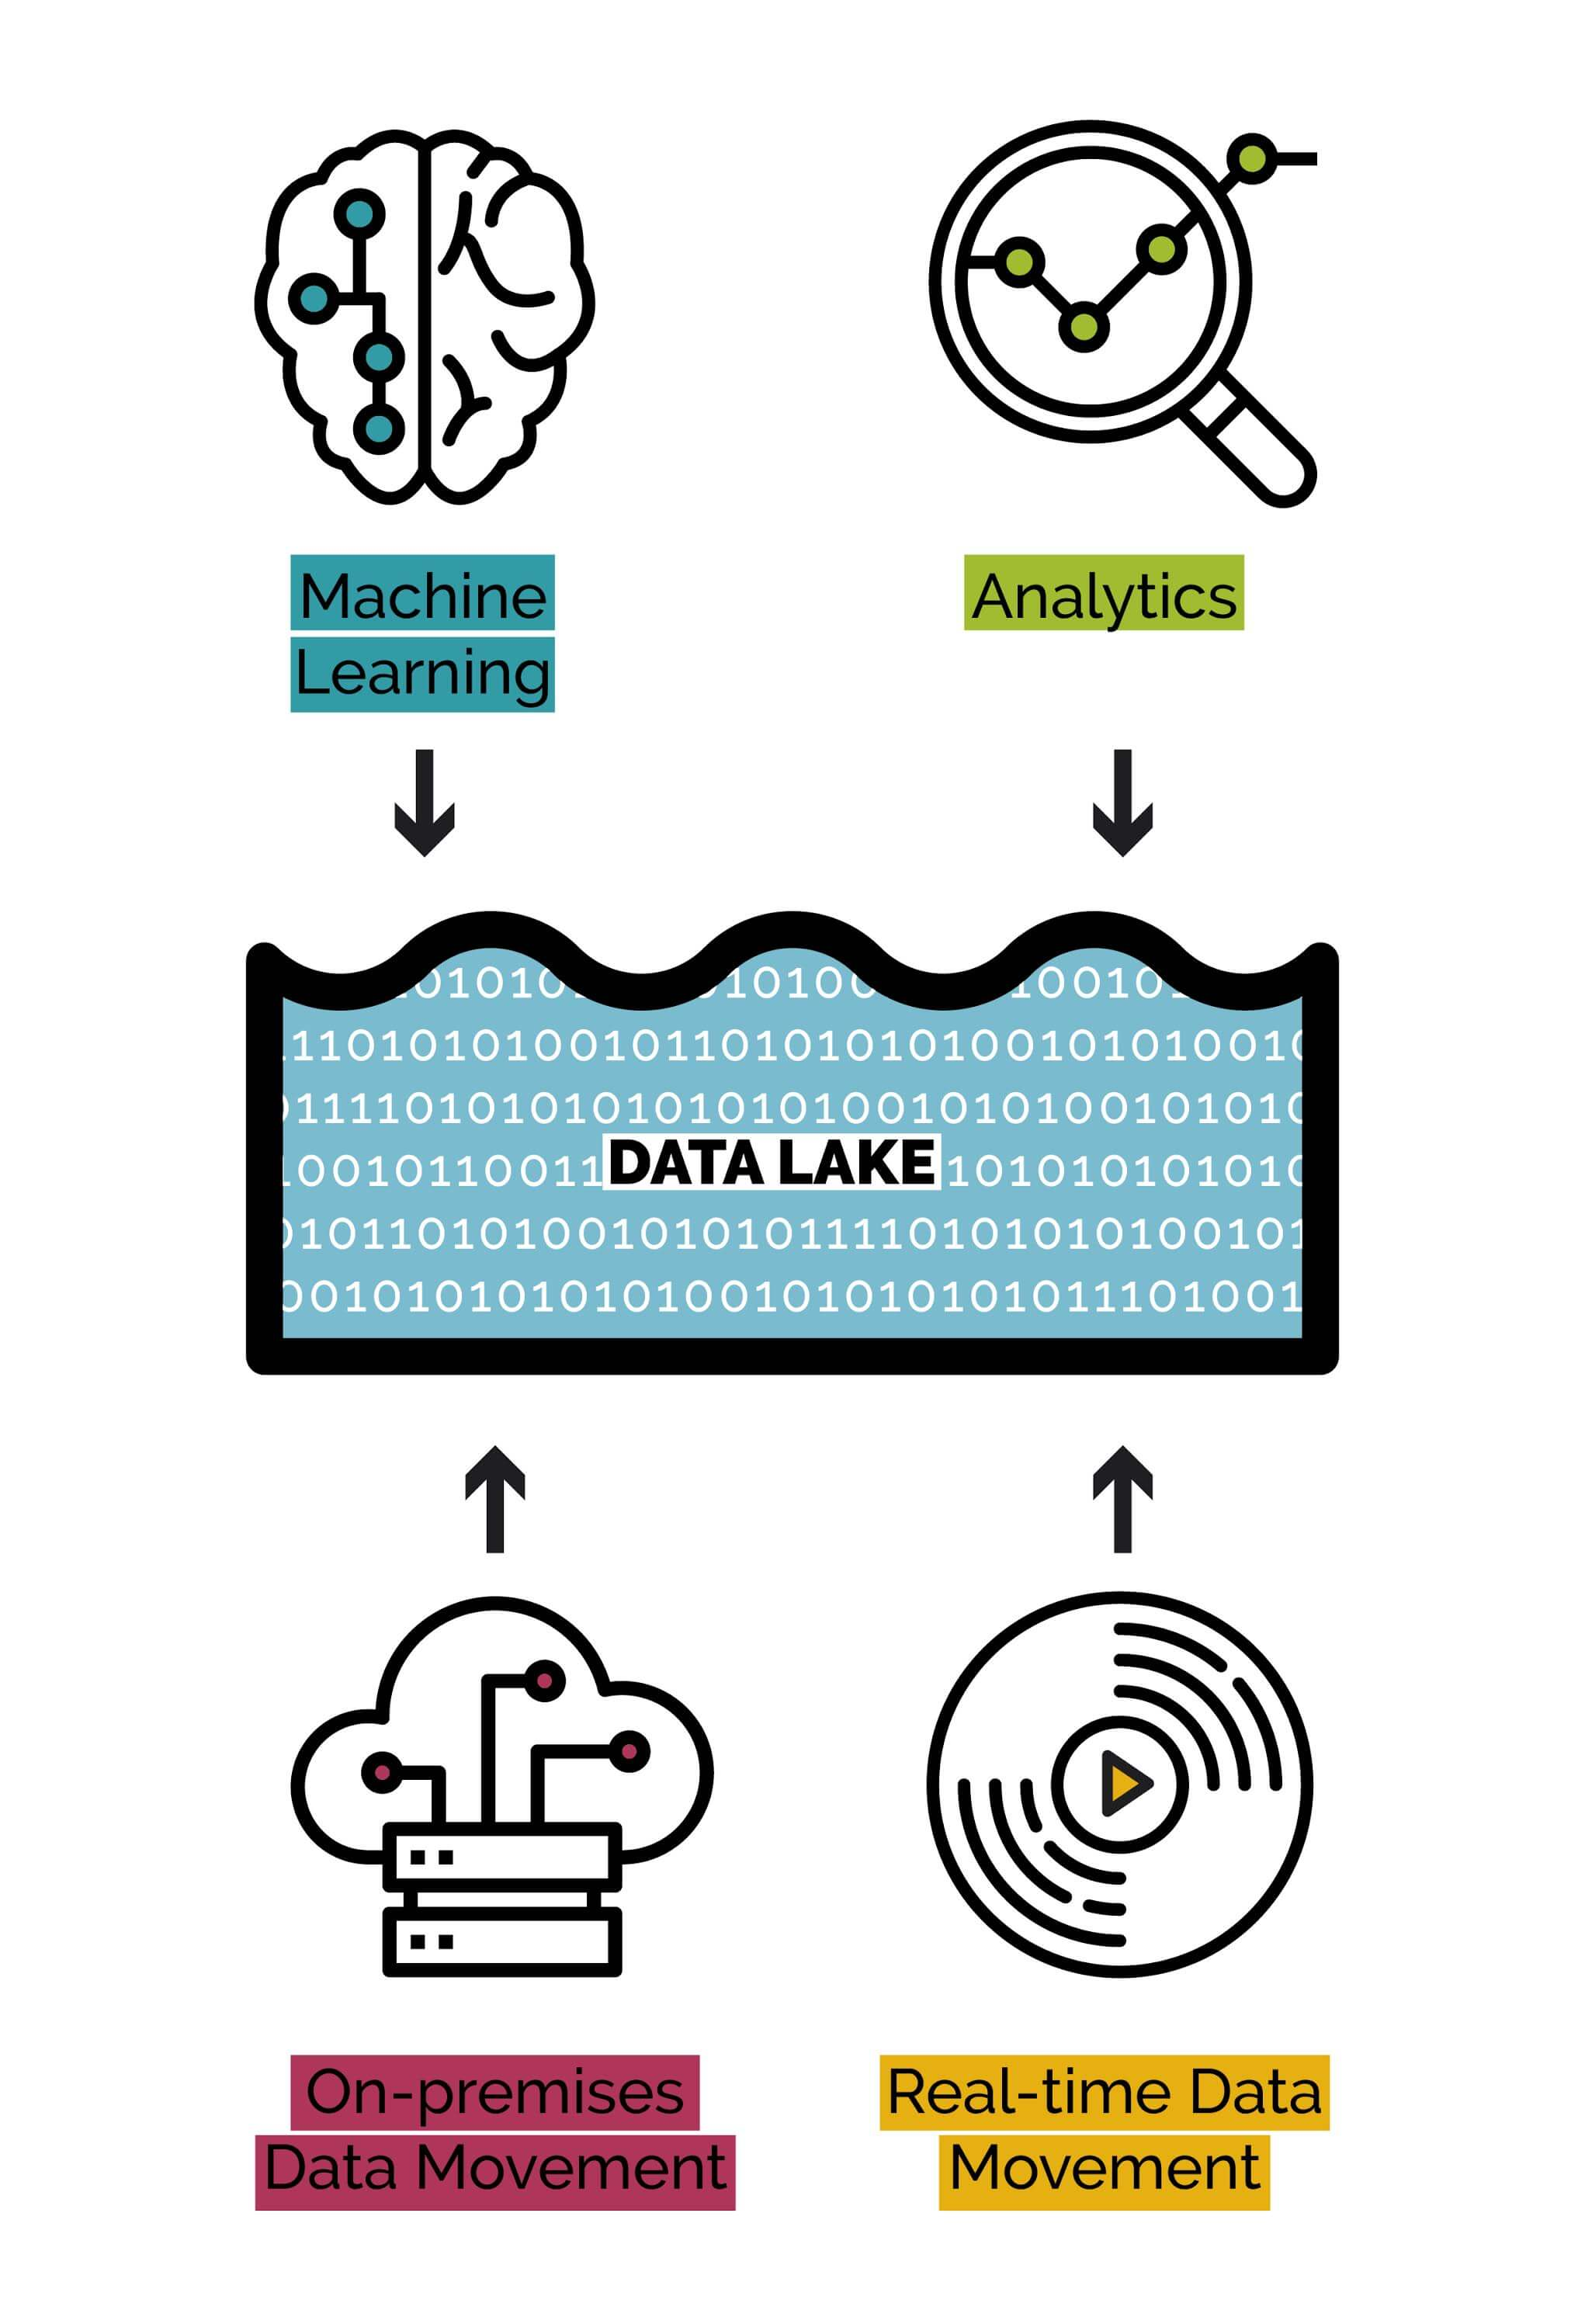
\includegraphics[width=10cm]{./IMAGENES/datalake}
				\end{center}
			\end{figure}
%-------------------------------------------------
\subsection{COMPONENTES DE DATALAKES}

\begin{itemize}
	\item \textbf{ Ingestión y almacenamiento de datos:}Es la capacidad de adquirir datos en tiempo real o en lotes, y también es la capacidad de almacenar datos y hacerlos accesibles.
	\item  \textbf{Procesamiento de datos:} Es la capacidad de trabajar datos sin procesar para que puedan analizarse a través de procesos estándar. 
También tiene la función de soluciones de ingeniería, que pueden extraer valor de los datos utilizando procesos regulares y automáticos generados por las operaciones de análisis.
	\item  \textbf{ Análisis de datos:} Es la creación de módulos para extraer información de los datos de manera sistemática; esto puede suceder en tiempo real o mediante un proceso que se ejecuta periódicamente.
	\item  \textbf{Integración de datos:} es la capacidad de conectar aplicaciones a la plataforma; En primer lugar, las aplicaciones deben permitir consultar el Data Lake para extraer los datos en el formato correcto, en función del uso que desee hacer de ellos.
\end{itemize}

%-------------------------------------------------
\subsection{DATALAKES *********}

Ralph Kimball, plantea la idea de un enfoque dimensional para el diseño de un DW, y afirma que la unión de todos los DM de una organización constituye el DW corporativo, a lo cual se le conoce como el enfoque bottom-up.\\

%-------------------------------------------------

\subsection{COMPARACION DE DATAWAREHOUSE Y DATALAKES}	
\begin{figure}[htb]
				\begin{center}
					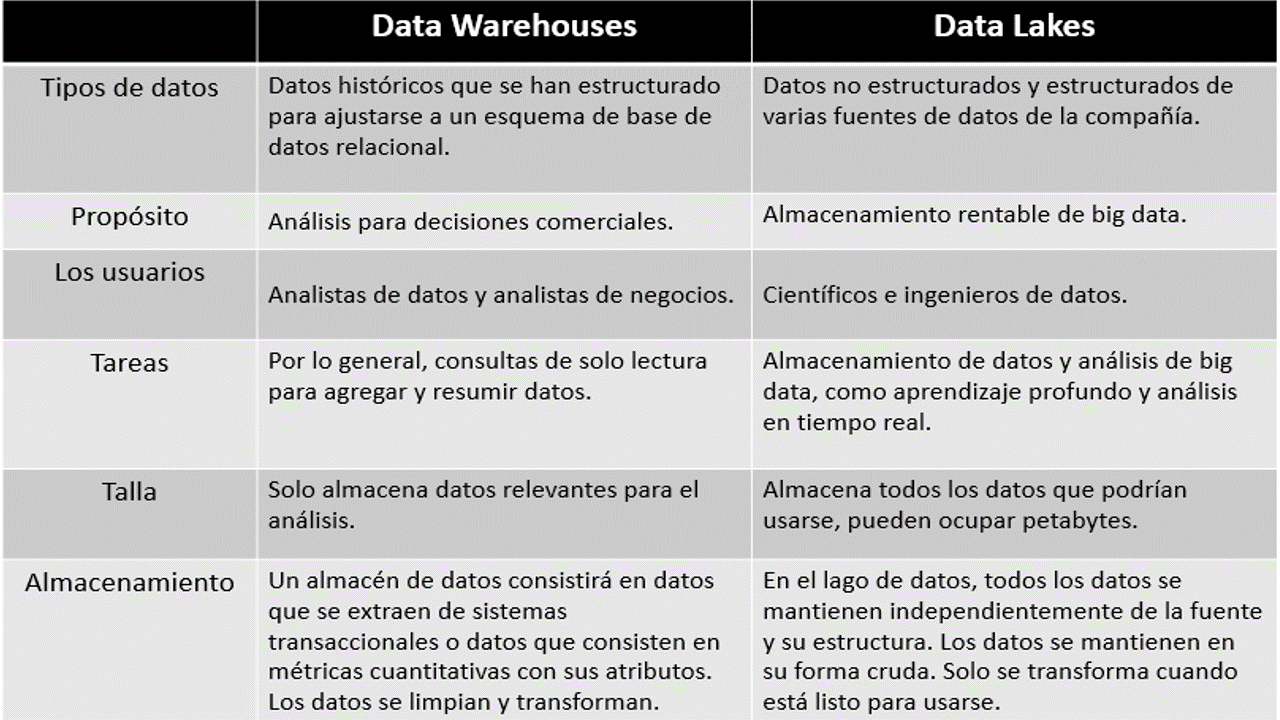
\includegraphics[width=10cm]{./IMAGENES/Imagen1}
				\end{center}
			\end{figure}
%-----------------------------------------------------------------
\section{Conclusiones}

\begin{itemize}
\item Es necesario revisar la categorías de un lago de datos y un almacén de datos, para analizar cual se adapta mejor al caso de uso en el que se desea trabajar.
\item Cuando se construyen tuberías de datos, es necesario implementar una combinación de ambas soluciones de almacenamiento.
\item El lago de datos integran diferentes tipos de datos para generar preguntas completamente nuevas, ya que es probable que estos usuarios no usen almacenes de datos porque pueden necesitar ir más allá de sus capacidades, mientras que en el almacén de datos la mayoría de los usuarios de una organización están operativos. Este tipo de usuarios solo se preocupa por los informes y las métricas clave de rendimiento.

\end{itemize}


% Bibliografia.
%-----------------------------------------------------------------

\bibliographystyle{apalike}

\bibliography{Bibliografia}

\end{document}
